%\begin{figure}[h!]
%\begin{center} 
%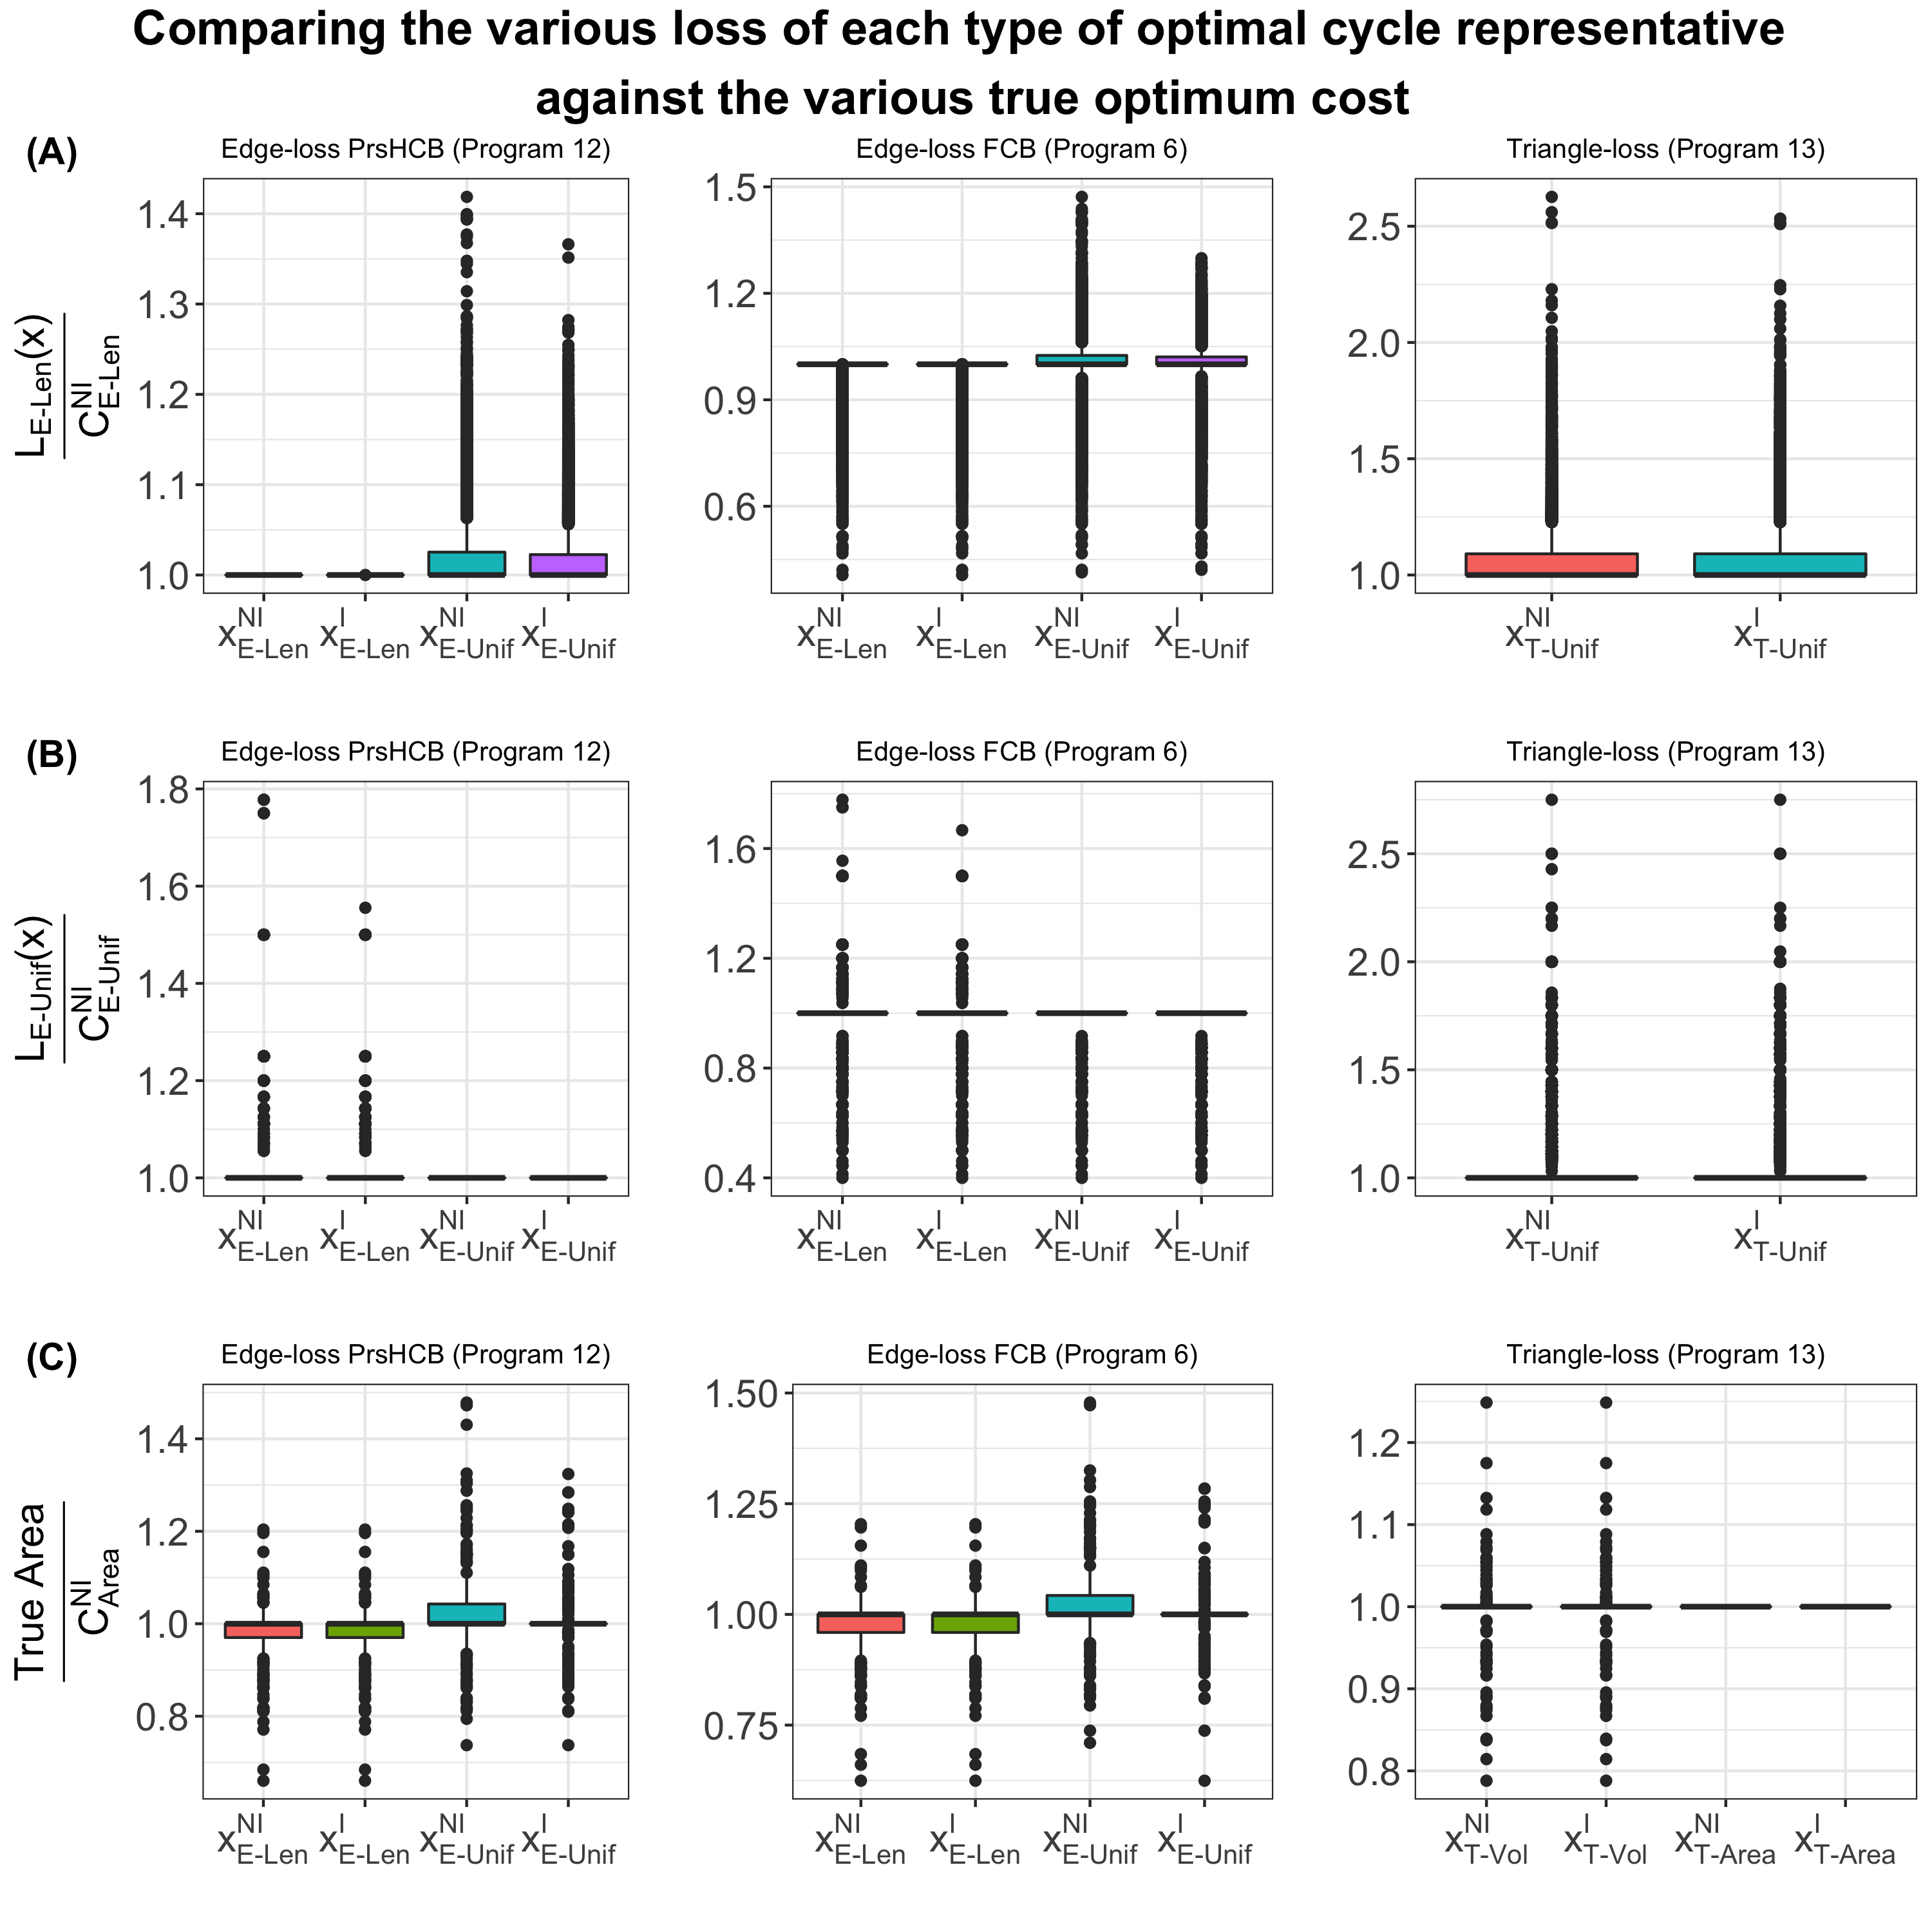
\includegraphics[width=\textwidth]{figures/length_area_edge.png}
%\end{center}
%\caption{Box plot comparing the enclosed area of each type of optimal cycle representative against the optimum area-weighted volume optimal cost. These data aggregate $190$ cycle representatives from $10$ point clouds from a normal distribution with ambient dimension of $2$. True area represents the total area enclosed by the representative, while $C_{Area}\NI$ represents the area of the area-weighted volume optimal cycle minimizing \ref{eq:LP-Area}. We observe that some uniform/length-weighted optimal cycles have an area smaller than that of the area-weighted volume optimal cycle. Refer to Figure \ref{fig:areaExample} to see why this may happen. In addition to $\optimalrep_{Area}\NI = \optimalrep_{Area}\I$ for corresponding cycle representatives in all experiments, so too are $\optimalrep_{Len}\NI = %\optimalrep_{Len}\I$\LZ{Remove, right??}}\label{fig:areacompare}
%\end{figure}
